%% OK con Grammarly

\section{Methodology}
The project's methodology is detailed in two steps. First, the project's action plan is laid out and explained. Then, a timeline is presented with the work distribution and weekly milestones.

\subsection{Project phases}

The proposed analysis will be structured into five phases shown in Figure \ref{fig:plan_accion}. In this section, the work to be performed is defined in each of the five steps. Section \ref{cronograma} provides finer details regarding the timeline of each step.


\begin{figure}[h!]
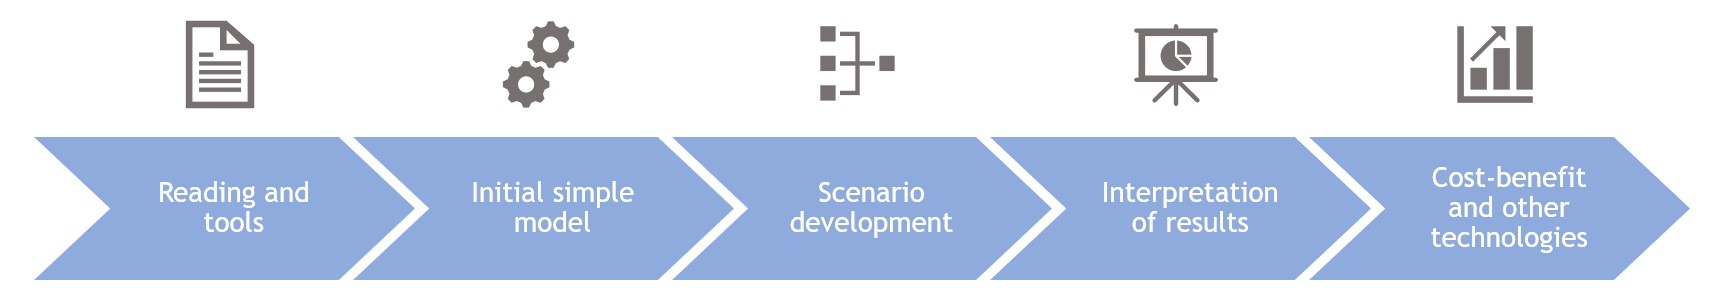
\includegraphics[width=\textwidth]{images/metodologia_trabajo_1.jpg}
\caption{Proposed action plan}
\label{fig:plan_accion}
\centering
\end{figure}


\begin{description}
   \item[Reading and tools.] Read PRIME 1.4 and standard 802.15.4 documentation. Investigation and documentation regarding the state of the art and related topics. Preparation of the OMNeT environment \cite{omnet} and the SimPRIME library \cite{simprime}. Understand the simulation tools, simulate simple scenarios, and ensure legacy code is working as intended.
   \item[Initial simple model.] Independent scenario testing of PRIME and RF technologies. Analyze the results separately and ensure they are in line with expected theoretical outcomes. After this has been achieved, join both scenarios to create a simple model where both technologies work as intended.
   \item[Scenario development.] Define which parameters to compare in the study. Once they have been defined, we will generalize and tweak the previous code to collect results according to the chosen parameter values (these values are defined in the following phase). The final goal of this step is to have a functional PRIME Hybrid simulation with the ability to introduce variable entry parameters.
   \item[Interpretation of results.] Gather all relevant information and characteristics of scenarios to simulate. With this information, parameter values will be defined to run the simulations. Their outcome will be analyzed.
    \item[Cost-benefit and other technologies.] The conclusions reached from comparing the various scenarios will be compared with high-level results from other technologies. In this step, a cost-benefit analysis will also be performed to further compare PRIME Hybrid with alternative network communication technologies.
\end{description}



\subsection{Timeline}\label{cronograma}

The project has an estimated duration of 34 weeks. The starting date is October 11th 2021. The project will end on the week of May 30th 2022 with the final project presentation. A Gantt diagram with the detailed timeline is presented at the end of the document.

